 \documentclass{article}
\usepackage[utf8]{inputenc}
\usepackage{float}
\usepackage{amsmath}
\usepackage[labelsep=period]{caption} % Figur. istället för Figur:
\usepackage{relsize}
\usepackage{multirow}
\usepackage[export]{adjustbox}
\usepackage{subcaption}
\usepackage{wrapfig}
\usepackage{hyperref}
\usepackage{array}
\usepackage{amsmath}
\usepackage{geometry}
\usepackage{parskip}
\newcommand\tab[1][1cm]{\hspace*{#1}}

\title{Reinforcement Learning EL2805\\
       Laboration 2}

\author{Ilian Corenliussen, 950418-2438, ilianc@kth.se\\ 
        Daniel Hirsch, 960202-5737, dhirsch@kth.se}
\date{December 2020}

\begin{document}

\maketitle

\section*{Problem 1: \\
        Deep Q-Networks (DQN)}
\subsection*{A)}

\subsection*{B)} In a DQN a replay buffer is used to stabilize the learning process. By mixing previous with new experience to make the network train on a mixed expenses rather then only consider new experience. This is done before the update of the neural network, to decorrelation the training samples for each batch. The target network is used to have a stable target values too compare to, instead of updating after every step we update at every $C$-step and thus we have a stable copy of the network(target network) too compare to.
\subsection*{C)}

\subsection*{D)}
We chose to implement a network with one hidden layer, the input layer uses $8$ neurons to match the 8-dimensional state of the problem. The hidden layer had the size of $50$ neurons. The optimizer chosen was the Adam optimizer as it was suggested for these types of problems. The clipping value was set to $1$.\\
\noindent The size of the experience replay buffer parameter $L$ was chosen to $20000$ after iterating through values between $5000 - 30000$. The parameter $N$, i.e. the size of the training batch were chosen to $24$ to match the complexity of our problem, as it generally is in the order of $4 - 128$.
The update frequency of the target network, $C$, were chosen to be $C = L/N$ as it is the general suggestion for the update frequency. The number of episodes $T_E$ where iterated between $100$ to $1000$, and the chosen value were $600$. The number of episodes were chosen to $600$ because no significant performance inrease where found for more episodes, also when training the neural network to long it starts forgetting. $\epsilon$ were chosen to exponentially decay between the values of $0.99$ and $0.05$. The discount factor $\gamma$ was set to $0.99$. 

\subsection*{E)}
\subsubsection*{1)}
As can be seen in Figure \ref{fig:Policy} the total reward goes up for the training and stops to decrease after approximately 580 episodes. The number of steps does also steady decrease after 200 episodes. Where the hyperparameters where selected as described under Section D.
\begin{figure}[H]
    \centering
    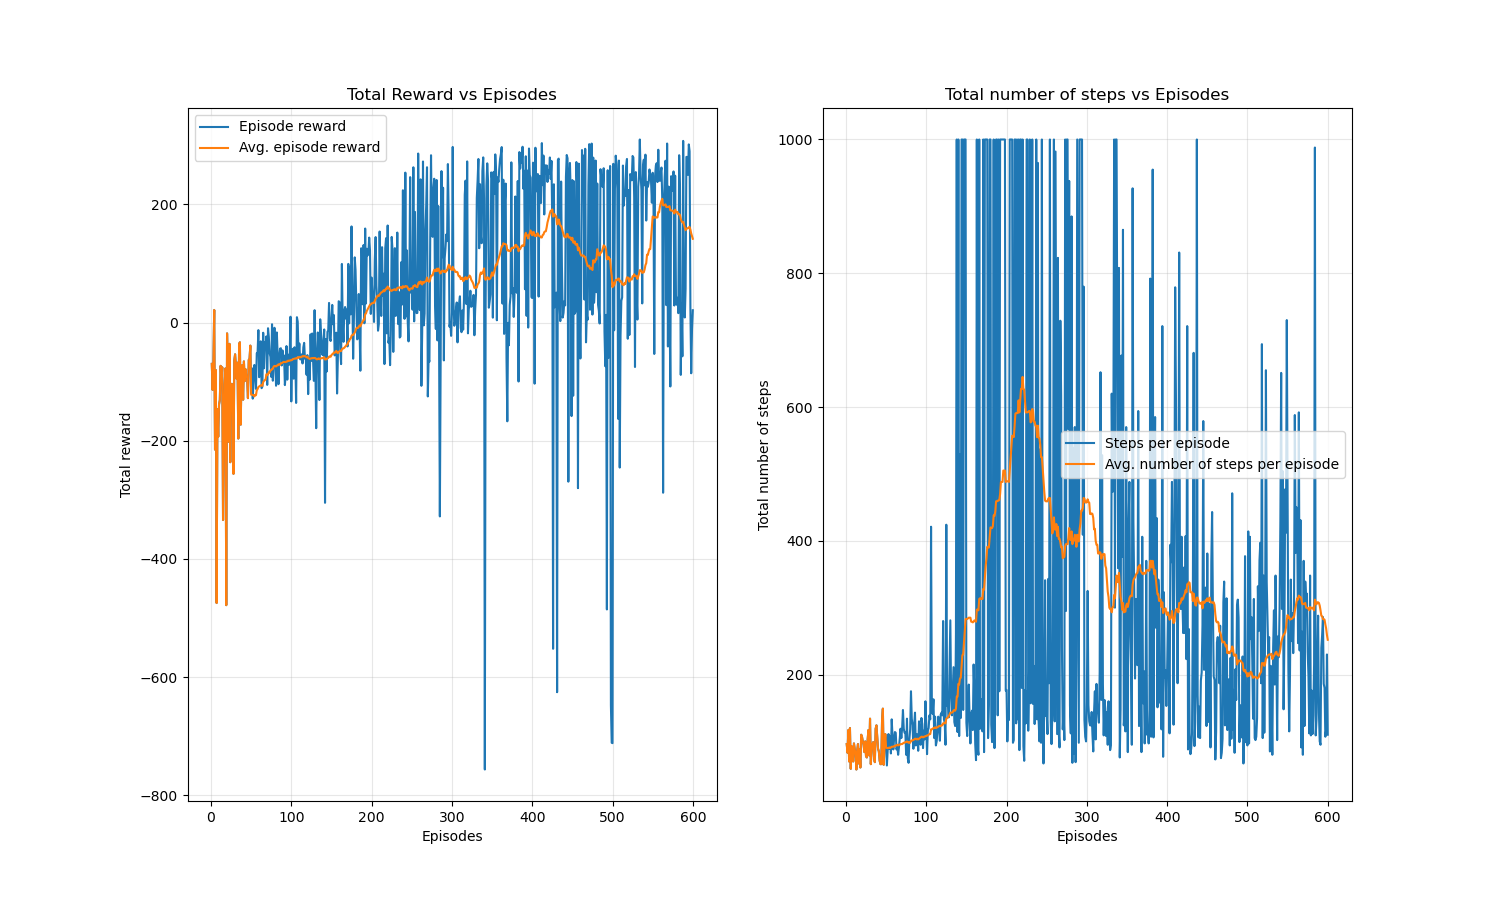
\includegraphics[width=1\textwidth]{Lab_2/problem1/images/main_network.png}
    \caption{\small Total episodic reward and the number of steps taken per episodes during training for the final optimized policy. }
    \label{fig:Policy}
\end{figure}

\subsubsection*{2)}
When using $\gamma_1$ the lander mostly took the approach of hovering, due to no punishment of rewards far in the future see Figure \ref{fig:gamma1}. A too low gamma, such as $\gamma_2$, the lander took a too aggressive approach of descent which resulted in a less satisfying reward score see Figure \ref{fig:gamma0.2}.
\begin{figure}[H]
    \centering
    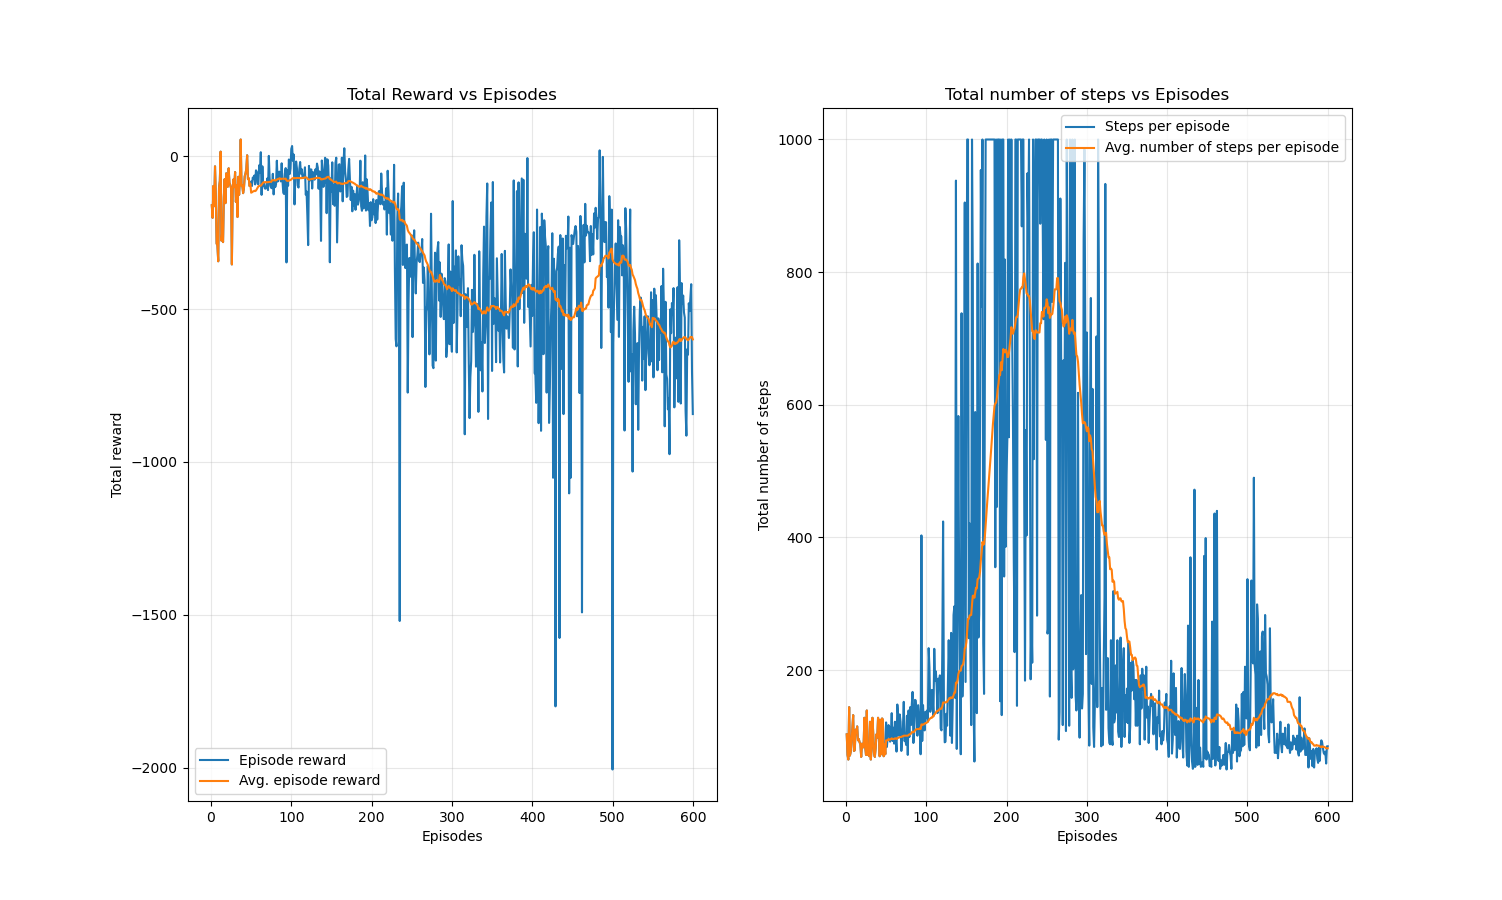
\includegraphics[width=1\textwidth]{Lab_2/problem1/images/gamma_1.png}
    \caption{\small Total episodic reward and the number of steps taken per episodes during training with $\gamma_1$. . }
    \label{fig:gamma1}
\end{figure}

\begin{figure}[H]
    \centering
    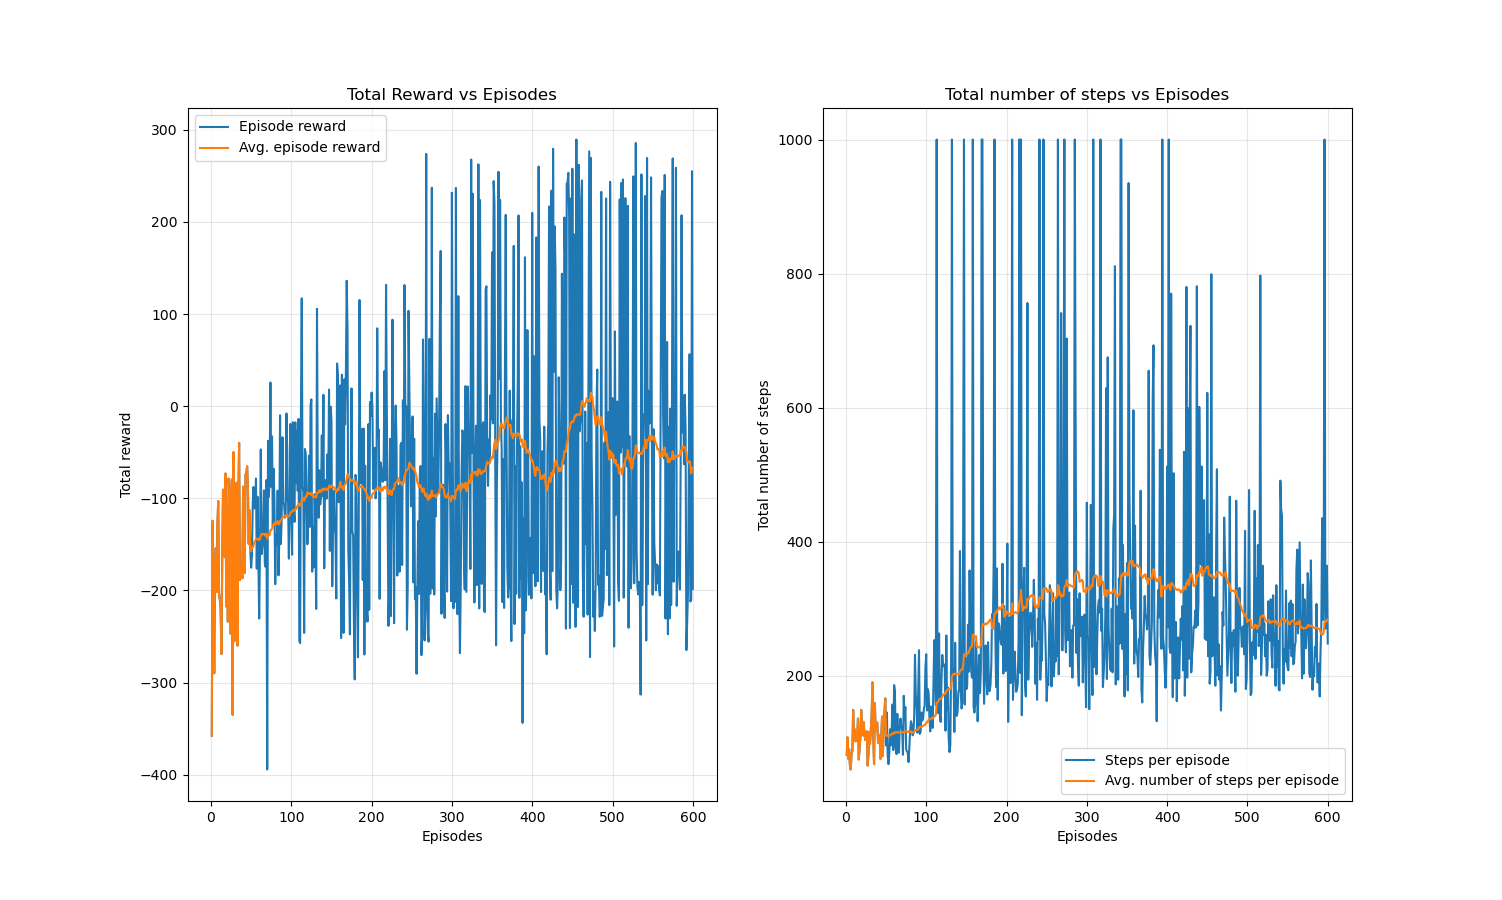
\includegraphics[width=1\textwidth]{Lab_2/problem1/images/gamma_02.png}
    \caption{\small Total episodic reward and the number of steps taken per episodes during training with $\gamma_2$. }
    \label{fig:gamma0.2}
\end{figure}

\subsubsection*{3)}
When using 1000 episodes the average reward does not decrease, i.e. no catastrophic memory loss, but it does not have any significant improvement either see Figure \ref{fig:episodes1000}. When increasing the buffer size to $5000$, a decrease in the average reward is obtained, see Figure \ref{fig:buffer5000}. The training process also seems to be more stable, at least for the first $350$ episodes. But it fluctuates more in its behaviours due to it more frequently fills its buffer with new experiences.  
\begin{figure}[H]
    \centering
    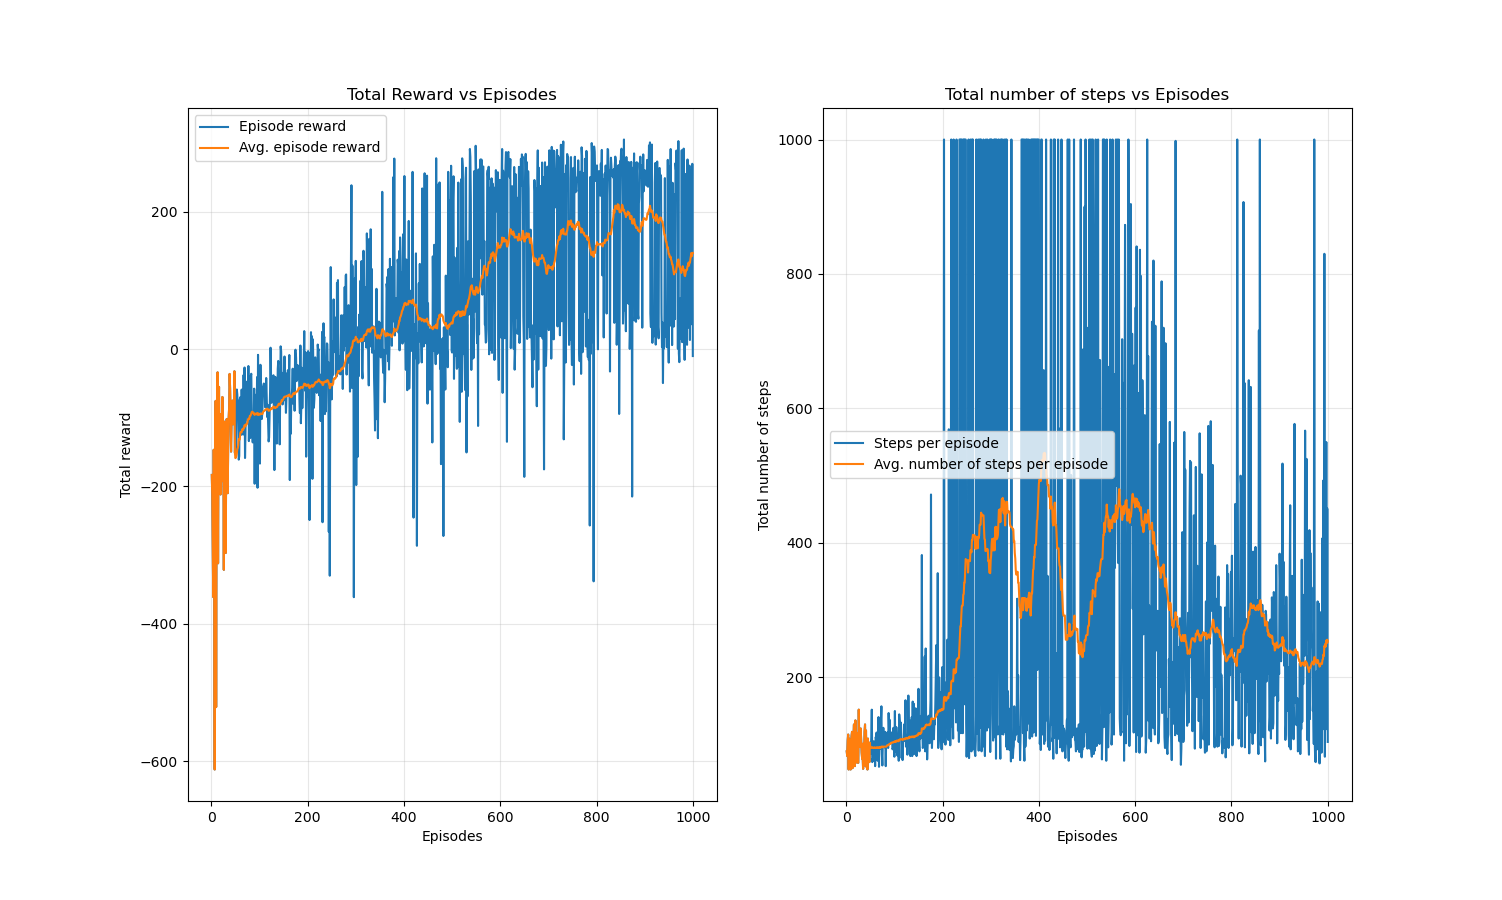
\includegraphics[width=1\textwidth]{Lab_2/problem1/images/episodes1000.png}
    \caption{\small Total episodic reward and the number of steps taken per episodes during training, trained for 1000 episodes. }
    \label{fig:episodes1000}
\end{figure}


\begin{figure}[H]
    \centering
    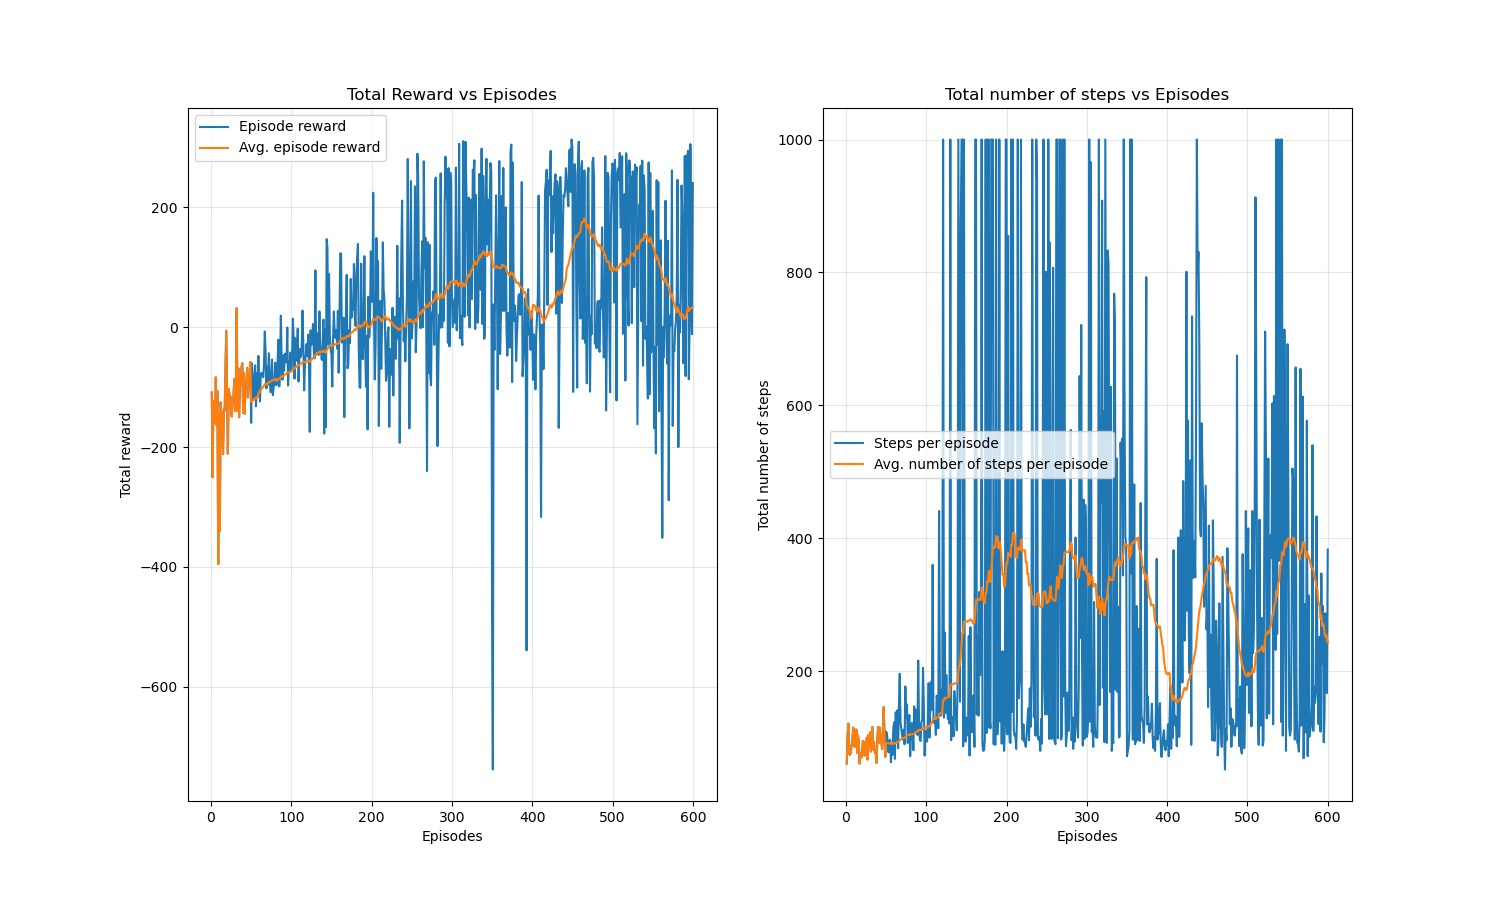
\includegraphics[width=1\textwidth]{Lab_2/problem1/images/buffer5000.png}
    \caption{\small Total episodic reward and the number of steps taken per episodes during training, trained for 1000 episodes. With a buffer size of $5000$. }
    \label{fig:buffer5000}
\end{figure}


\subsection*{F)}
\begin{figure}[H]
    \centering
    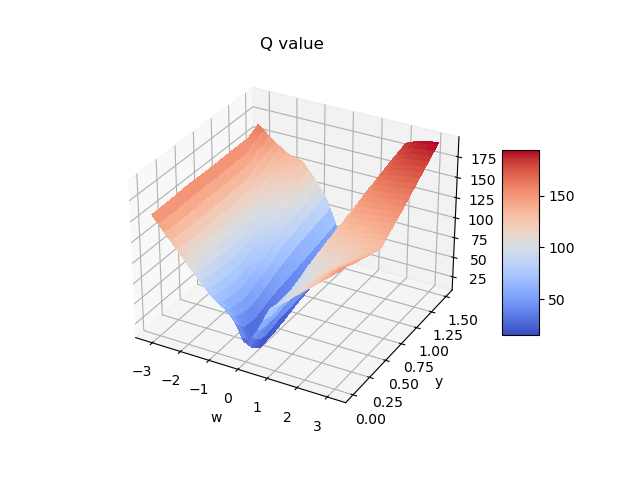
\includegraphics[width=1\textwidth]{Lab_2/problem1/images/Q_value.png}
    \caption{\small FILL IN}
    \label{fig:Q_value}
\end{figure}

\subsection*{G)}
\begin{figure}[H]
    \centering
    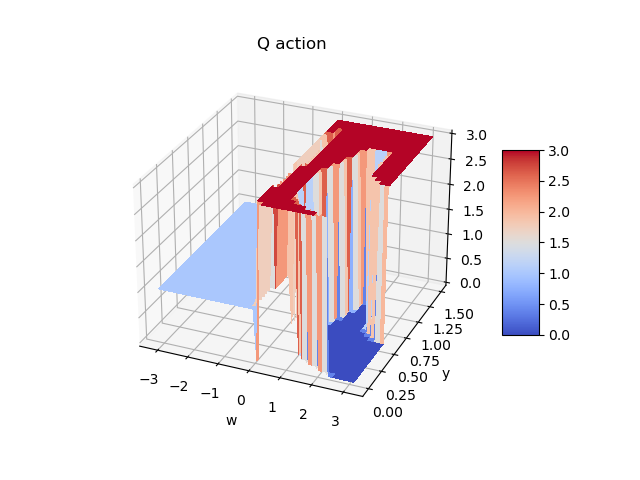
\includegraphics[width=1\textwidth]{Lab_2/problem1/images/Q_action.png}
    \caption{\small FILL IN }
    \label{fig:Q_action}
\end{figure}

\subsection*{H)}
\begin{figure}[H]
    \centering
    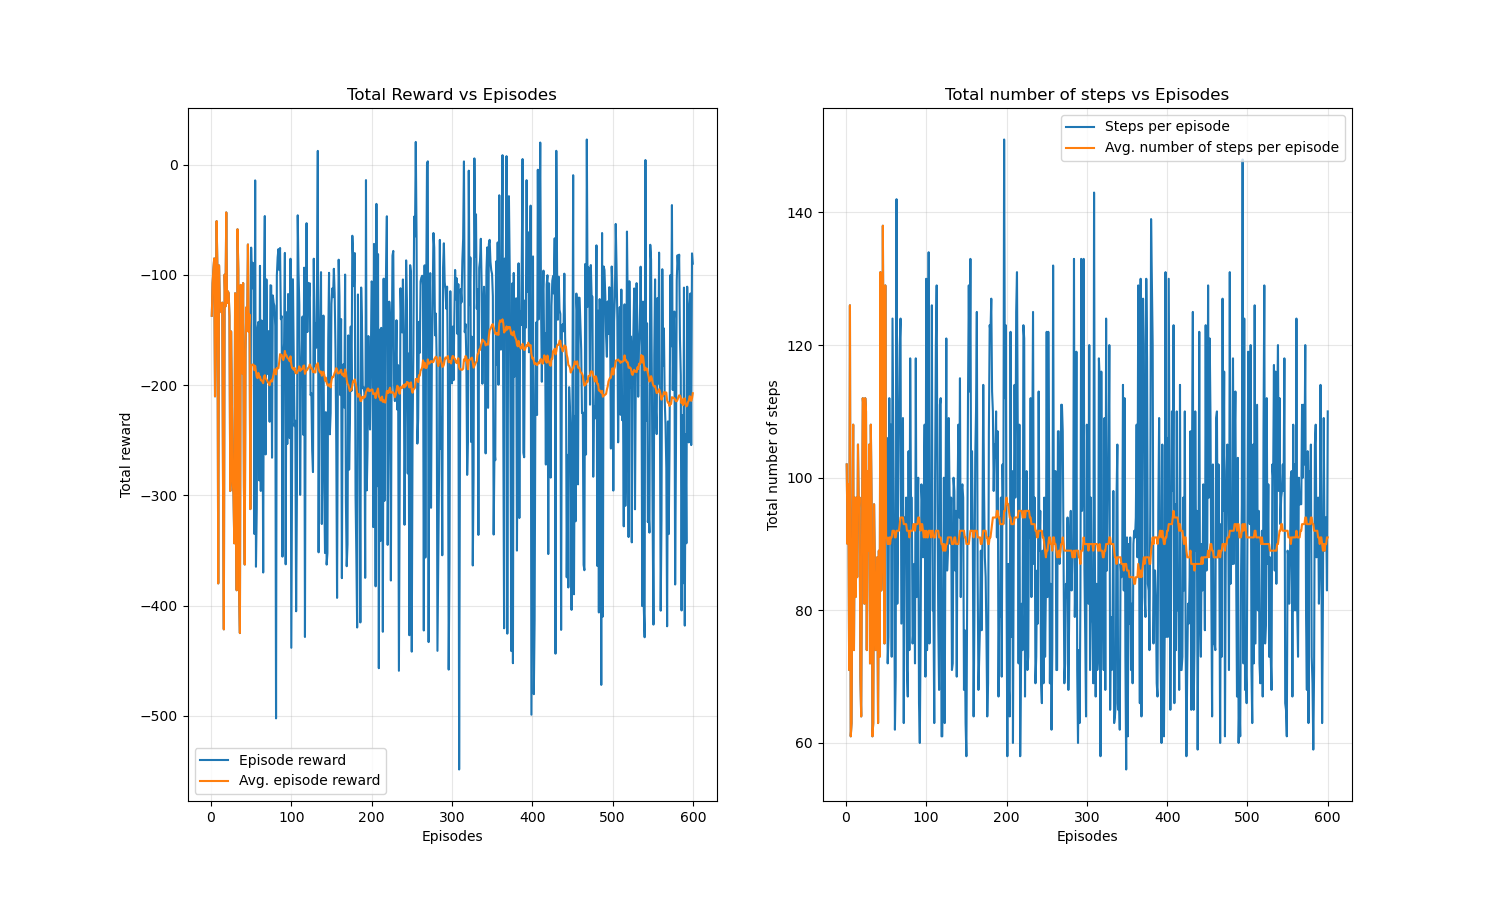
\includegraphics[width=1\textwidth]{Lab_2/problem1/images/randomAgent.png}
    \caption{\small FILL IN }
    \label{fig:randomAgent}
\end{figure}



\end{document}
